\providecommand{\norm}[1]{\left\lVert #1 \right\rVert}

\chapter{Matrix Operations}

In Part~6, we used adjacency matrices and distance tables to capture network connectivity. Here in Part~7, we shift from combinatorial graph traversals to numerical and algebraic computation.

Somewhere in your past a teacher drew a grid of numbers, called it a
``matrix,'' and made you multiply two of them by a procedure that felt like a
secret handshake: go across one, down the other, add up the products. You did
it, but you may never have paused to ask the deeper question:
\emph{why is multiplication defined this way, and what geometric transformation does it represent?}

This chapter answers both. We will rebuild matrices as a tool for computation. A matrix, it turns out, is the natural language for
talking about \emph{many things changing at once}: a thousand linear equations,
a rotation in space, a step of a neural network, the flow of populations between
cities. The operations we study --- multiply, decompose, solve, invert --- are
the verbs of that language, and they are central to
scientific computing, graphics, statistics, optimization, and machine learning.

\begin{focusbox}
Matrix operations translate systems of linear equations and geometric transformations into fast algorithms. Through LUP decomposition, triangular substitution, Strassen's subcubic multiplication, and matrix inversion, we solve linear systems in $O(n^3)$ time and demonstrate that matrix inversion is asymptotically equivalent to matrix multiplication.
\end{focusbox}

\section{Matrices from the ground up}

A \emph{matrix} is a rectangular array of numbers. We write $A$ for the whole
array and $a_{ij}$ for the entry in row $i$, column $j$. A matrix with $m$ rows
and $n$ columns is an ``$m \times n$ matrix'' (always rows first, columns
second --- say it out loud a few times so the order sticks). A matrix with one
column is a \emph{column vector}; one row, a \emph{row vector}. When $m=n$ we call
the matrix \emph{square}.

$$
A=\begin{pmatrix} 2 & 0 & 1\\ 3 & 5 & 4 \end{pmatrix}
\quad\text{is } 2\times 3,\qquad a_{13}=1,\quad a_{21}=3.
$$

Two matrices of the same shape \emph{add} entrywise: $(A+B)_{ij}=a_{ij}+b_{ij}$.
You scale a matrix by a number $c$ entrywise too: $(cA)_{ij}=c\,a_{ij}$. Both cost
$\Th(mn)$ time --- one operation per entry, no surprises. The interesting verb is
multiplication. (See Appendix~42 for further foundations on vector spaces and matrix properties.)

\subsection{Why multiplication is defined the way it is}

One idea explains the ``secret handshake.'' Think of an
$m\times n$ matrix not just as a static grid of numbers, but as a linear map
that takes an input vector of length $n$ and produces an output vector of
length $m$. Feed it the vector
$x=(x_1,\dots,x_n)$; out comes $y=Ax$, where
$$
y_i=\sum_{k=1}^{n} a_{ik}\,x_k .
$$
Row $i$ of $A$ is a recipe: ``to make output $i$, take $a_{i1}$ of the first
input plus $a_{i2}$ of the second, and so on.'' This is exactly how a system of
linear equations looks, and it is exactly how a layer of a neural network mixes
its inputs. A matrix \emph{is} a linear transformation written down in
coordinates.

Now suppose you have two machines. Machine $B$ ($n\times p$) turns a length-$p$
vector into a length-$n$ vector; machine $A$ ($m\times n$) turns that into a
length-$m$ vector. Chain them: first $B$, then $A$. The combined machine takes
length $p$ to length $m$. \emph{What single matrix represents the chained
machine?} Call it $C=AB$. Push a vector $x$ through: $z=Bx$ has entries
$z_k=\sum_j b_{kj}x_j$, and then $y=Az$ has entries
$$
y_i=\sum_{k} a_{ik}z_k=\sum_{k}a_{ik}\sum_{j}b_{kj}x_j
   =\sum_{j}\Big(\underbrace{\sum_{k}a_{ik}b_{kj}}_{c_{ij}}\Big)x_j .
$$
The thing in the parentheses must be $c_{ij}$, because $y=Cx$ means
$y_i=\sum_j c_{ij}x_j$. So the definition is forced on us:
$$
\boxed{\,c_{ij}=\sum_{k=1}^{n}a_{ik}\,b_{kj}\,}
$$

\begin{intuitionbox}
Matrix multiplication is \emph{composition of machines}. The reason you go
``across a row of $A$ and down a column of $B$'' is that $c_{ij}$ collects every
path from input $j$, through some middle coordinate $k$, to output $i$: the
coefficient $b_{kj}$ on the way in, the coefficient $a_{ik}$ on the way out,
multiplied, then summed over all middles $k$. This is
the only rule that makes ``do $B$, then do $A$'' equal ``do $AB$.''
\end{intuitionbox}

Two shapes must match for the product to exist: the \emph{inner} dimensions. An
$m\times n$ times an $n\times p$ gives an $m\times p$. The $n$'s must agree
because the middle coordinate $k$ runs over them. Figure~\ref{ch27:rowcol}
shows which slice of each factor produces a single output entry.

\begin{figure}[h]
\centering
\begin{tikzpicture}[scale=0.62, every node/.style={font=\small}]
% A matrix, highlight row i
\draw (0,0) rectangle (3,3);
\node at (1.5,3.4) {$A$ ($m\times n$)};
\fill[sourceblue!30] (0,1.5) rectangle (3,2);
\node[sourceblue!60!black] at (-0.9,1.75) {row $i$};
% B matrix, highlight column j
\draw (4.5,0) rectangle (7.5,3);
\node at (6,3.4) {$B$ ($n\times p$)};
\fill[targetgreen!30] (5.5,0) rectangle (6,3);
\node[targetgreen!60!black] at (5.75,-0.45) {col $j$};
% C matrix, highlight entry ij
\draw (9,0) rectangle (12,3);
\node at (10.5,3.4) {$C=AB$ ($m\times p$)};
\fill[quotientorange!40] (10,1.5) rectangle (10.5,2);
\node[quotientorange!60!black] at (10.25,0.95) {$c_{ij}$};
% arrow
\draw[-Latex,gray!70] (7.7,1.75) .. controls (8.4,1.75) and (8.4,1.75) .. (8.95,1.75);
\node[font=\footnotesize] at (6.0,-2.1)
  {$c_{ij}=\displaystyle\sum_{k}a_{ik}\,b_{kj}$ (row $i$ of $A$ dotted with col $j$ of $B$)};
\end{tikzpicture}
\caption{The entry $c_{ij}$ of the product gathers row $i$ of $A$ against
column $j$ of $B$. The shared length $n$ is the ``inner'' dimension both factors
must agree on.}
\label{ch27:rowcol}
\end{figure}

\begin{example}[A product, traced by hand]
\label{ch27:product-trace}
Let
$$
A=\begin{pmatrix}1 & 2\\ 3 & 4\end{pmatrix},\qquad
B=\begin{pmatrix}5 & 6\\ 7 & 8\end{pmatrix}.
$$
Both are $2\times 2$, so $C=AB$ is $2\times 2$. Compute each entry by
``row of $A$ dotted with column of $B$'':
\begin{align*}
c_{11}&=1\cdot 5+2\cdot 7=5+14=19, &
c_{12}&=1\cdot 6+2\cdot 8=6+16=22,\\
c_{21}&=3\cdot 5+4\cdot 7=15+28=43, &
c_{22}&=3\cdot 6+4\cdot 8=18+32=50.
\end{align*}
So $C=\begin{pmatrix}19 & 22\\ 43 & 50\end{pmatrix}$. Notice $BA$ is
\emph{different}: $BA=\begin{pmatrix}23 & 34\\ 31 & 46\end{pmatrix}$. Matrix
multiplication does \emph{not} commute --- of course not: putting on socks then
shoes is not the same as shoes then socks.
\end{example}

\begin{trapbox}
Three traps that bite everyone at least once.
\textbf{(1) Order matters.} $AB\ne BA$ in general; you may not silently swap.
\textbf{(2) Shapes must line up.} You can multiply $A$ ($m\times n$) by $B$
($n\times p$) only when $A$'s column count equals $B$'s row count. ``$2\times 3$
times $2\times 3$'' is undefined.
\textbf{(3) Indices.} $c_{ij}$ uses row $i$ of $A$ and column $j$ of $B$. Going
``down a column of $A$'' by accident is the single most common bug in handwritten
matrix code.
\end{trapbox}

A few special matrices earn names. The \emph{identity} $I_n$ has $1$'s on the
diagonal and $0$'s elsewhere; it is the ``do nothing'' machine, so $AI=IA=A$. The
\emph{transpose} $A^{\mathsf T}$ flips rows and columns:
$(A^{\mathsf T})_{ij}=a_{ji}$. A matrix is \emph{symmetric} if $A=A^{\mathsf T}$.
A \emph{diagonal} matrix is zero off the diagonal; \emph{lower triangular} means
zero above the diagonal, \emph{upper triangular} means zero below. Keep
triangular matrices in mind --- the second half of this
chapter relies on them, because systems involving them can be solved directly by single-pass substitution.

\subsection{The cost of the schoolbook product}

How long does it take to multiply two $n\times n$ matrices by the definition? The
output has $n^2$ entries. Each entry is a sum of $n$ products. So we do
$n^2\cdot n=n^3$ scalar multiplications and about as many additions.

\begin{algorithm}[H]
\caption{\textsc{Square-Matrix-Multiply}$(A,B)$}
\KwIn{Two $n\times n$ matrices $A$ and $B$.}
\KwOut{Their product $C=AB$.}
let $C$ be a new $n\times n$ matrix\;
\For{$i\gets 1$ \KwTo $n$}{
  \For{$j\gets 1$ \KwTo $n$}{
    $c_{ij}\gets 0$\;
    \For{$k\gets 1$ \KwTo $n$}{
      $c_{ij}\gets c_{ij}+a_{ik}\cdot b_{kj}$\;
    }
  }
}
\Return $C$\;
\end{algorithm}

Three nested loops, each running $n$ times, with constant work inside: the
running time is $\Th(n^3)$. For decades people assumed that was the end of the
story --- surely you cannot multiply two matrices without touching every pair of
entries the cubic number of times. In 1969 Volker Strassen proved that
assumption wrong, and we turn to his trick next.

\begin{complexitybox}
\textbf{Schoolbook $n\times n$ matrix multiply.}
Scalar multiplications: $n^3$. Additions: $n^3-n^2$. Time: $\Th(n^3)$. Extra
space: $\Th(n^2)$ for the output (the inputs are read-only). Simple, cache-
friendly, and for small or medium $n$ it is genuinely the fastest thing you can
do.
\end{complexitybox}

\section{Strassen's algorithm, revisited}

You met divide-and-conquer earlier in the book. Applied to matrix
multiplication, it gives a surprising result.

\subsection{A first attempt: blocking}

Split each $n\times n$ matrix into four $n/2\times n/2$ \emph{blocks} (assume $n$
is a power of two so the halving stays clean):
$$
A=\begin{pmatrix}A_{11} & A_{12}\\ A_{21} & A_{22}\end{pmatrix},\quad
B=\begin{pmatrix}B_{11} & B_{12}\\ B_{21} & B_{22}\end{pmatrix},\quad
C=\begin{pmatrix}C_{11} & C_{12}\\ C_{21} & C_{22}\end{pmatrix}.
$$
\begin{figure}[h]
\centering
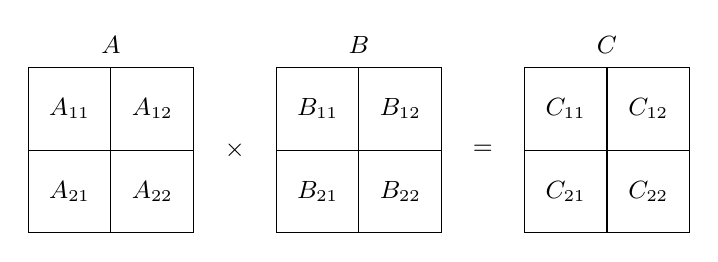
\begin{tikzpicture}[scale=0.7, every node/.style={font=\small}]
\foreach \xo/\lab in {0/A, 4.5/B, 9/C}{
  \draw (\xo,0) rectangle (\xo+3,3);
  \draw (\xo+1.5,0)--(\xo+1.5,3);
  \draw (\xo,1.5)--(\xo+3,1.5);
  \node at (\xo+1.5,3.4) {$\lab$};
  \node at (\xo+0.75,2.25) {$\lab_{11}$};
  \node at (\xo+2.25,2.25) {$\lab_{12}$};
  \node at (\xo+0.75,0.75) {$\lab_{21}$};
  \node at (\xo+2.25,0.75) {$\lab_{22}$};
}
\node at (3.75,1.5) {$\times$};
\node at (8.25,1.5) {$=$};
\end{tikzpicture}
\caption{Each $n\times n$ matrix is split into four $n/2\times n/2$ blocks. The
blocks then multiply by the same ``rows times columns'' rule as scalar entries,
e.g.\ $C_{11}=A_{11}B_{11}+A_{12}B_{21}$.}
\label{ch27:blocks}
\end{figure}

Blocks multiply by the same rule as scalars, as long as
you keep the order straight (see Figure~\ref{ch27:blocks}). So
$$
\begin{aligned}
C_{11}&=A_{11}B_{11}+A_{12}B_{21}, & C_{12}&=A_{11}B_{12}+A_{12}B_{22},\\
C_{21}&=A_{21}B_{11}+A_{22}B_{21}, & C_{22}&=A_{21}B_{12}+A_{22}B_{22}.
\end{aligned}
$$
Each of the four output blocks is a sum of two products of half-size matrices:
$8$ multiplications of $n/2\times n/2$ matrices, plus a handful of $n/2\times n/2$
additions (each costing $\Th(n^2)$). That gives the recurrence
$$
T(n)=8\,T(n/2)+\Th(n^2).
$$
By the master theorem (here $a=8$, $b=2$, so $n^{\log_b a}=n^{\log_2 8}=n^3$, and
the $\Th(n^2)$ combine is polynomially smaller), $T(n)=\Th(n^3)$. We split the
work cleverly and \emph{got nothing}: still cubic. The eight multiplications are
the problem. Strassen's insight is to do the same job with \emph{seven}.

\subsection{Seven products instead of eight}

Strassen discovered that you can compute the four output blocks using only
\emph{seven} multiplications of half-size matrices, at the cost of a few extra
additions and subtractions. The additions are cheap ($\Th(n^2)$); the
multiplications are the expensive recursive calls, so trading one multiplication
for several additions is a clear win. First form ten sums:
$$
\begin{aligned}
S_1&=B_{12}-B_{22}, & S_2&=A_{11}+A_{12}, & S_3&=A_{21}+A_{22},\\
S_4&=B_{21}-B_{11}, & S_5&=A_{11}+A_{22}, & S_6&=B_{11}+B_{22},\\
S_7&=A_{12}-A_{22}, & S_8&=B_{21}+B_{22}, & S_9&=A_{11}-A_{21},\\
S_{10}&=B_{11}+B_{12}. & & & &
\end{aligned}
$$
Then the seven products (these are the recursive multiplications):
$$
\begin{aligned}
P_1&=A_{11}\,S_1, & P_2&=S_2\,B_{22}, & P_3&=S_3\,B_{11}, & P_4&=A_{22}\,S_4,\\
P_5&=S_5\,S_6, & P_6&=S_7\,S_8, & P_7&=S_9\,S_{10}. & &
\end{aligned}
$$
Finally assemble the answer with additions and subtractions only:
$$
\begin{aligned}
C_{11}&=P_5+P_4-P_2+P_6, & C_{12}&=P_1+P_2,\\
C_{21}&=P_3+P_4, & C_{22}&=P_5+P_1-P_3-P_7.
\end{aligned}
$$

\begin{intuitionbox}
Do not try to \emph{memorize} those formulas, and do not expect them to be
immediately apparent --- they are not. The structural point is that by
allowing yourself to add and subtract input blocks \emph{before} multiplying, you
can arrange for the products to overlap so much that seven of them carry all the
information eight used to. It is the same spirit as the fast Fourier transform:
spend cheap operations (adds) to save expensive ones (multiplies).
\end{intuitionbox}

Let us check one entry explicitly to see how the cancellation works.

\begin{example}[Verifying $C_{12}=P_1+P_2$]
\label{ch27:strassen-check}
$P_1=A_{11}S_1=A_{11}(B_{12}-B_{22})=A_{11}B_{12}-A_{11}B_{22}$, and
$P_2=S_2B_{22}=(A_{11}+A_{12})B_{22}=A_{11}B_{22}+A_{12}B_{22}$. Adding,
$$
P_1+P_2=A_{11}B_{12}-A_{11}B_{22}+A_{11}B_{22}+A_{12}B_{22}
       =A_{11}B_{12}+A_{12}B_{22}=C_{12}.
$$
The two $A_{11}B_{22}$ terms cancel exactly. Strassen's formulas work this
way throughout: a term you do not want is created in one product and cancelled in another.
\end{example}

\subsection{Why seven beats eight: the recurrence}

The recurrence is now
$$
T(n)=7\,T(n/2)+\Th(n^2).
$$
Here $a=7$, $b=2$, so $n^{\log_b a}=n^{\log_2 7}$. Since $\log_2 7\approx 2.807>2$,
the recursive term dominates the $\Th(n^2)$ combine, and the master theorem gives
$$
T(n)=\Th\!\big(n^{\log_2 7}\big)=\Th\!\big(n^{2.807\ldots}\big).
$$
That single dropped multiplication moved the exponent from $3.000$ down to about
$2.807$. The change looks small, but for $n=1024$, $n^3\approx 1.07\times 10^9$
while $n^{2.807}\approx 2.0\times 10^8$, roughly a fivefold reduction, and the gap
widens without bound as $n$ grows.

\begin{labbox}
\textbf{Trace the recursion tree.} At depth $d$ from the top there are $7^d$
subproblems, each of size $n/2^d$, and each does $\Th((n/2^d)^2)$ addition work.
So level $d$ costs $7^d\cdot c\,(n/2^d)^2=c\,n^2(7/4)^d$. The levels form a
geometric series with ratio $7/4>1$, so the \emph{bottom} levels dominate. There
are $\log_2 n$ levels, and the last level's cost is
$c\,n^2(7/4)^{\log_2 n}=c\,n^{\log_2 7}$. Sum the geometric series and the total is
$\Th(n^{\log_2 7})$. Draw this tree on paper for $n=8$: a root, $7$ children, $49$
grandchildren, and watch the per-level cost climb by $7/4$ each step.
\end{labbox}

\begin{figure}[h]
\centering
\begin{tikzpicture}[
  level distance=14mm,
  every node/.style={font=\small},
  edge from parent/.style={draw,gray!60,-Latex}]
\node[draw,rounded corners,fill=blue!6] (r) {$T(n)$: $1$ mult, size $n$}
  child {node[draw,rounded corners,fill=green!6] {$T(n/2)$}}
  child {node[draw,rounded corners,fill=green!6] {$T(n/2)$}}
  child {node {$\cdots$}}
  child {node[draw,rounded corners,fill=green!6] {$T(n/2)$}};
\node[anchor=west,font=\footnotesize\itshape,gray!60!black]
  at ($(r)+(2.4,0)$) {7 children, not 8};
\end{tikzpicture}
\caption{One level of Strassen's recursion: \emph{seven} subproblems of half the
size. Eight would give $\Th(n^3)$; seven gives $\Th(n^{2.807})$.}
\label{ch27:strassen-tree}
\end{figure}

\begin{historybox}
The computational study of matrices traces back to Carl Friedrich Gauss, who around 1801 used systematic row elimination to compute the celestial orbit of the asteroid Ceres from sparse astronomical observations. In 1948, Alan Turing formalized matrix decompositions and analyzed the propagation of roundoff errors in Gaussian elimination on digital computers. For decades, it was widely presumed that multiplying two $n \times n$ matrices inherently required $\Theta(n^3)$ operations. In 1969, Volker Strassen disproved this assumption in his paper ``Gaussian Elimination is not Optimal,'' presenting a clever decomposition that multiplies $2 \times 2$ block matrices using only 7 multiplications instead of 8, lowering the asymptotic complexity to $O(n^{\log_2 7}) \approx O(n^{2.807})$.

Strassen's discovery triggered intense debate between numerical analysts and theoreticians. Practical implementers observed that Strassen's algorithm exhibits less numerical stability than standard elimination under finite-precision floating-point arithmetic and incurs significant memory allocation overhead. Consequently, modern high-performance libraries (such as BLAS and LAPACK) continue to rely on block-partitioned Gaussian elimination with partial pivoting for moderate matrix dimensions.

On the theoretical side, Strassen's work led to the result that matrix multiplication, matrix inversion, and determinant computation are computationally equivalent, all bounded by the matrix multiplication exponent $\omega$. Don Coppersmith and Shmuel Winograd achieved $O(n^{2.376})$ in 1990 using the laser method, and ongoing refinements by Virginia Vassilevska Williams, Josh Alman, and others have reduced the upper bound near $2.371$. The fundamental open question remains whether $\omega = 2$ is achievable---whether multiplying two $n \times n$ matrices can be done in essentially $O(n^2)$ time. In 2014, Ambainis, Filmus, and Le Gall proved structural barrier limits on the laser method, indicating that reaching $\omega = 2$ will require entirely new mathematical techniques. In CLRS (4th edition), Strassen's algorithm appears in Chapter~4 and matrix operations in Chapter~28.
\end{historybox}

\begin{trapbox}
Strassen is \emph{not} a free lunch in practice. The extra additions, the
recursive bookkeeping, and worse numerical stability mean that on real hardware
Strassen only pays off for fairly large $n$ (often several hundred and up), and
serious libraries switch to the cache-tuned cubic algorithm once the blocks get
small. ``Asymptotically faster'' and ``faster on your laptop today'' are
different claims; respect the constant factors.
\end{trapbox}

\section{Solving linear systems: $Ax=b$}

Now we arrive at the operation that matrices were arguably invented for: solving
\emph{simultaneous linear equations}. You want $x$ such that $Ax=b$, where $A$ is
a known $n\times n$ matrix, $b$ a known vector, and $x$ the unknown vector. Spelled
out, that is $n$ equations in $n$ unknowns:
$$
\begin{aligned}
a_{11}x_1+a_{12}x_2+\cdots+a_{1n}x_n&=b_1,\\
&\ \,\vdots\\
a_{n1}x_1+a_{n2}x_2+\cdots+a_{nn}x_n&=b_n.
\end{aligned}
$$
You learned to do this with Gaussian elimination: scale and subtract rows until
the system is triangular, then read off the answers. We are going to repackage
exactly that process into a reusable \emph{factorization}, which is both cleaner
to reason about and far more useful when you must solve many systems with the same
$A$.

\begin{intuitionbox}
\textbf{Prerequisites: rank, determinant, and invertibility.}
When does a linear system $Ax=b$ have a unique solution? Linear algebra provides three equivalent perspectives:
\begin{itemize}
  \item \textbf{Rank}: The rank of $A$ is the maximum number of linearly independent columns (or rows). A square $n \times n$ matrix has \emph{full rank} $n$ precisely when no row is a redundant combination of others, meaning each equation provides genuinely independent information.
  \item \textbf{Determinant}: The determinant $\det(A)$ measures the signed $n$-dimensional volume scaling factor under the transformation $x \mapsto Ax$. If $\det(A) = 0$, the matrix squashes space into a lower dimension, destroying information and preventing a unique pre-image. If $\det(A) \ne 0$, the transformation is non-degenerate and volume is preserved with finite non-zero scaling. In an LUP decomposition, $\det(A) = (-1)^s \prod_{i=1}^n u_{ii}$, where $s$ is the number of row swaps in $P$ and $u_{ii}$ are the diagonal pivots of $U$.
  \item \textbf{Inverse}: If $A$ has full rank ($\det(A) \ne 0$), there exists a unique two-sided inverse matrix $A^{-1}$ satisfying $A A^{-1} = A^{-1} A = I_n$.
\end{itemize}
\end{intuitionbox}

\subsection{Triangular systems are easy}

Start with the easy case, because the whole strategy is ``reduce the hard case to
the easy one.'' Suppose $A$ is \emph{lower triangular} (zeros above the diagonal).
Then the first equation involves only $x_1$, so you solve it immediately. The
second involves $x_1$ (now known) and $x_2$, so you solve for $x_2$. Marching down,
each new equation introduces exactly one new unknown. This is \emph{forward
substitution}:
$$
x_i=\frac{1}{\ell_{ii}}\Big(b_i-\sum_{j=1}^{i-1}\ell_{ij}\,x_j\Big).
$$
For an \emph{upper} triangular system you start from the \emph{last} equation and
march up --- \emph{back substitution}. Either way the cost is $\Th(n^2)$: roughly
one multiply-add per nonzero entry below (or above) the diagonal.

\begin{example}[Forward substitution by hand]
\label{ch27:forward-sub}
Solve $Lx=b$ with
$$
L=\begin{pmatrix}2 & 0 & 0\\ 1 & 3 & 0\\ 4 & 5 & 6\end{pmatrix},\qquad
b=\begin{pmatrix}4\\ 11\\ 40\end{pmatrix}.
$$
Row 1: $2x_1=4\Rightarrow x_1=2$.
Row 2: $1\cdot 2+3x_2=11\Rightarrow 3x_2=9\Rightarrow x_2=3$.
Row 3: $4\cdot 2+5\cdot 3+6x_3=40\Rightarrow 8+15+6x_3=40\Rightarrow 6x_3=17$,
so $x_3=17/6$. Each step uses only already-known values --- no system-solving, just
arithmetic.
\end{example}

\subsection{LU and LUP decomposition}

Here is the plan. Most matrices are not triangular, but \emph{every} (nonsingular)
matrix can be \emph{factored} into a product of triangular matrices. If we can
write
$$
A=LU,\qquad L \text{ unit lower triangular},\ U \text{ upper triangular},
$$
then $Ax=b$ becomes $L(Ux)=b$. Let $y=Ux$. First solve $Ly=b$ by forward
substitution (easy, triangular), then solve $Ux=y$ by back substitution (easy,
triangular). Two easy solves replace one hard one. ``Unit'' lower triangular means
$L$ has $1$'s on its diagonal --- a normalization that makes the factorization
unique.

Where does $L$ come from? It is the \emph{record of Gaussian elimination}. When you
eliminate $x_1$ from row $i$ by subtracting a multiple $\ell_{i1}$ of row 1, you
\emph{store} that multiplier $\ell_{i1}$. Collect all the multipliers into $L$ and
the eliminated (upper-triangular) result into $U$, and you can check that $LU=A$.
No information is lost: the multipliers in $L$ record every step.

\begin{intuitionbox}
LU decomposition is Gaussian elimination that \emph{records its row multipliers}. The
upper-triangular $U$ is where elimination leaves the matrix. The lower-triangular
$L$ records, in entry $\ell_{ij}$, exactly how much of row $j$ you subtracted from
row $i$ along the way. Multiply $L$ back into $U$ and
you recover the original $A$. The factorization stores the result of the algorithm
so that it can be reused.
\end{intuitionbox}

One catch makes the plain $A=LU$ recipe fragile: at some step the entry we want to
divide by (the \emph{pivot}) might be zero, or merely tiny. Dividing by a tiny
pivot amplifies rounding error catastrophically. The fix is \emph{pivoting}: before
each elimination step, swap rows to bring the largest-magnitude available entry into
the pivot position. Swapping rows is itself a matrix operation --- multiplication by
a \emph{permutation matrix} $P$ --- and recording all the swaps gives the more robust
\emph{LUP decomposition}:
$$
PA=LU.
$$
Now solving $Ax=b$ becomes: permute $b$ to get $Pb$, forward-solve $Ly=Pb$,
back-solve $Ux=y$. Same two easy solves, just with the rows reordered first.

\begin{focusbox}
\textbf{The LUP strategy.} Factor once: $PA=LU$, costing
$\Th(n^3)$. Then \emph{each} right-hand side $b$ is solved for $\Th(n^2)$ by a
forward solve and a back solve. If you must solve $Ax=b$ for many different $b$'s
with the same $A$, you pay the cubic cost a single time and the cheap quadratic
cost over and over.
\end{focusbox}

\begin{example}[A full LU factorization]
\label{ch27:lu-example}
Factor (no pivoting needed here)
$$
A=\begin{pmatrix}2 & 4 & -2\\ 4 & 9 & -3\\ -2 & -3 & 7\end{pmatrix}.
$$
\textbf{Step 1: eliminate column 1.} Pivot is $a_{11}=2$.
Multiplier for row 2: $\ell_{21}=4/2=2$; subtract $2\times$row 1 from row 2:
$(4,9,-3)-2(2,4,-2)=(0,1,1)$.
Multiplier for row 3: $\ell_{31}=-2/2=-1$; subtract $-1\times$row 1 from row 3:
$(-2,-3,7)-(-1)(2,4,-2)=(0,1,5)$.
The matrix is now $\begin{pmatrix}2&4&-2\\0&1&1\\0&1&5\end{pmatrix}$.

\textbf{Step 2: eliminate column 2.} Pivot is $1$. Multiplier
$\ell_{32}=1/1=1$; subtract $1\times$row 2 from row 3:
$(0,1,5)-(0,1,1)=(0,0,4)$. Now the matrix is upper triangular:
$$
U=\begin{pmatrix}2 & 4 & -2\\ 0 & 1 & 1\\ 0 & 0 & 4\end{pmatrix},\qquad
L=\begin{pmatrix}1 & 0 & 0\\ 2 & 1 & 0\\ -1 & 1 & 1\end{pmatrix}.
$$
Check: $LU$ should rebuild $A$. Row 3 of $LU$ is
$(-1)(2,4,-2)+(1)(0,1,1)+(1)(0,0,4)=(-2,-3,7)$, the original row 3. It works.
\end{example}

\begin{algorithm}[H]
\caption{\textsc{LUP-Decomposition}$(A)$}
\KwIn{A nonsingular $n\times n$ matrix $A$.}
\KwOut{A permutation $\pi$ and matrices $L,U$ (stored in $A$) with $PA=LU$.}
let $\pi[1\ldots n]$ be a new array; \For{$i\gets 1$ \KwTo $n$}{$\pi[i]\gets i$}
\For{$k\gets 1$ \KwTo $n$}{
  $p\gets 0$\;
  \For{$i\gets k$ \KwTo $n$}{
    \If{$\abs{a_{ik}}>p$}{$p\gets \abs{a_{ik}}$; \ $k'\gets i$\tcp*{find largest pivot}}
  }
  \lIf{$p=0$}{\textbf{error} ``singular matrix''}
  exchange $\pi[k]\leftrightarrow\pi[k']$ and row $k\leftrightarrow$ row $k'$ of $A$\;
  \For{$i\gets k+1$ \KwTo $n$}{
    $a_{ik}\gets a_{ik}/a_{kk}$\tcp*{store multiplier in $L$'s slot}
    \For{$j\gets k+1$ \KwTo $n$}{
      $a_{ij}\gets a_{ij}-a_{ik}\cdot a_{kj}$\tcp*{eliminate}
    }
  }
}
\Return $\pi$\;
\end{algorithm}

\begin{figure}[h]
\centering
\begin{tikzpicture}[
  scale=0.92,
  every node/.style={font=\small},
  lbl/.style={font=\scriptsize\scshape, text=gray!80!black}
]
  % Panel A: Factorization Structure PA = LU
  \draw[rounded corners=4pt, fill=gray!3, draw=gray!25] (-1.0, 0.4) rectangle (12.2, 4.2);
  \node[lbl, anchor=west] at (-0.8, 3.9) {Structural Factorization: $P \cdot A = L \cdot U$};

  % P matrix
  \node at (0.2, 2.2) {$\begin{pmatrix} 0 & 1 & 0 \\ 1 & 0 & 0 \\ 0 & 0 & 1 \end{pmatrix}$};
  \node[lbl] at (0.2, 0.75) {$P$ (Permute)};

  \node at (1.55, 2.2) {$\cdot$};

  % A matrix
  \node at (2.85, 2.2) {$\begin{pmatrix} a_{11} & a_{12} & a_{13} \\ a_{21} & a_{22} & a_{23} \\ a_{31} & a_{32} & a_{33} \end{pmatrix}$};
  \node[lbl] at (2.85, 0.75) {$A$ (Original)};

  \node at (4.25, 2.2) {$=$};

  % L matrix
  \node at (5.75, 2.2) {$\begin{pmatrix} 1 & 0 & 0 \\ \ell_{21} & 1 & 0 \\ \ell_{31} & \ell_{32} & 1 \end{pmatrix}$};
  \node[lbl, text=targetgreen!80!black] at (5.75, 0.75) {$L$ (Unit Lower)};

  \node at (7.3, 2.2) {$\cdot$};

  % U matrix
  \node at (8.95, 2.2) {$\begin{pmatrix} u_{11} & u_{12} & u_{13} \\ 0 & u_{22} & u_{23} \\ 0 & 0 & u_{33} \end{pmatrix}$};
  \node[lbl, text=sourceblue!80!black] at (8.95, 0.75) {$U$ (Upper Tri)};

  % Panel B: Two-Stage Solve Pipeline & In-Place Packing
  \draw[rounded corners=4pt, fill=sourceblue!2, draw=sourceblue!25] (-1.0, -2.4) rectangle (12.2, -0.1);
  \node[lbl, anchor=west] at (-0.8, -0.35) {Solving Pipeline \& In-Place Array Packing};

  % Solve flow
  \node[draw, rounded corners=2pt, fill=white, thick, align=center, font=\small] (pb) at (0.4, -1.25) {Permute\\$b \mapsto Pb$};
  \node[draw, rounded corners=2pt, fill=targetgreen!15, thick, align=center, font=\small] (ly) at (3.8, -1.25) {Forward Solve\\$Ly = Pb$};
  \node[draw, rounded corners=2pt, fill=sourceblue!15, thick, align=center, font=\small] (ux) at (7.6, -1.25) {Back Solve\\$Ux = y$};
  \node[draw, rounded corners=2pt, fill=quotientorange!20, thick, align=center, font=\small] (sol) at (10.8, -1.25) {Solution\\vector $x$};

  \draw[->, >=stealth, very thick, gray!70] (pb) -- (ly);
  \draw[->, >=stealth, very thick, gray!70] (ly) -- node[above=2pt, font=\tiny\bfseries, text=targetgreen!80!black] {vector $y$} (ux);
  \draw[->, >=stealth, very thick, gray!70] (ux) -- (sol);

  \node[font=\tiny\itshape, text=gray!70!black, anchor=west] at (-0.8, -2.1)
    {In-place packing: $L$'s sub-diagonal multipliers $\ell_{ik}$ and $U$'s upper entries $u_{kj}$ overwrite array $A$ directly ($\Theta(1)$ extra space).};
\end{tikzpicture}
\caption{Visual structure of LUP matrix decomposition. Top: row permutation $P$ stabilizes elimination, decomposing $PA$ into unit lower-triangular matrix $L$ and upper-triangular matrix $U$. Bottom: solving $Ax=b$ reduces to a two-step triangular pipeline (forward substitution $Ly=Pb$ followed by back substitution $Ux=y$) taking $\Theta(n^2)$ time per right-hand side $b$. In-place execution packs both $L$ and $U$ within the original array $A$.}
\label{ch27:lupack}
\end{figure}

A space-saving detail (Figure~\ref{ch27:lupack}): $L$ and $U$ never overlap
(off-diagonal $L$ below, $U$ on and above the diagonal, and $L$'s diagonal $1$'s
are implicit), so both fit inside the original array $A$. No extra $\Th(n^2)$
storage needed.

\begin{complexitybox}
\textbf{LUP decomposition.} The outer loop runs $n$ times; step $k$ does about
$(n-k)^2$ multiply-adds in its double inner loop. Summing,
$\sum_{k=1}^{n}(n-k)^2\approx n^3/3$, so the time is $\Th(n^3)$ ---
asymptotically the same as one matrix multiply, with a smaller constant.
\textbf{Each solve} afterward (forward + back substitution) is $\Th(n^2)$.
Pivot search adds only $\Th(n^2)$ total, lost in the noise.
\end{complexitybox}

\begin{walkbox}
You need to solve $Ax=b_1$, $Ax=b_2$, \dots, $Ax=b_{1000}$ --- a thousand
right-hand sides, same $A$ ($n=500$). Estimate the work two ways: (a) solve each
from scratch with full elimination; (b) factor $A=LU$ once, then do a thousand
cheap solves. Which is faster, and by roughly what factor? (Hint: compare
$1000\cdot n^3/3$ against $n^3/3 + 1000\cdot n^2$.) This is why
linear-algebra libraries hand you a reusable \emph{factorization object} rather than
an ad-hoc solve routine.
\end{walkbox}

\subsection{Why we never compute $A^{-1}$ to solve $Ax=b$}

Beginners reach for the inverse: ``$Ax=b$, so $x=A^{-1}b$ --- just invert and
multiply!'' This is correct mathematically but a poor way to compute. Computing $A^{-1}$ costs
more than an LUP factorization, then you still must multiply $A^{-1}b$. And the
inverse is numerically worse: it tends to be denser and to amplify rounding error.
The factor-and-substitute route is faster \emph{and} more accurate. Compute
inverses only when you genuinely need the inverse \emph{matrix} itself, not merely
the solution to a system.

\section{Matrix inversion and its equivalence to multiplication}

The \emph{inverse} of a square matrix $A$ is the matrix $A^{-1}$ with
$AA^{-1}=A^{-1}A=I$. It exists exactly when $A$ is \emph{nonsingular} (its columns
are linearly independent; equivalently $\det A\ne 0$). The inverse is the ``undo''
machine: if $A$ turns $x$ into $b$, then $A^{-1}$ turns $b$ back into $x$.

\subsection{Computing the inverse with LUP}

You can read $A^{-1}$ off of solves. The $j$-th column of $A^{-1}$ is the solution
$x$ to $Ax=e_j$, where $e_j$ is the $j$-th standard basis vector (a $1$ in
position $j$, zeros elsewhere) --- because $AA^{-1}=I$ says ``$A$ times column $j$
of $A^{-1}$ equals column $j$ of $I$.'' So: factor $A=LU$ once ($\Th(n^3)$), then
solve $n$ systems $Ax=e_1,\dots,Ax=e_n$ ($n$ solves at $\Th(n^2)$ each, totaling
$\Th(n^3)$). Stack the $n$ answer vectors as columns and you have $A^{-1}$. Total
time: $\Th(n^3)$.

\begin{focusbox}
\textbf{Inversion costs the same order as multiplication: $\Th(n^3)$ by the
schoolbook route.} In fact, inversion and
multiplication are \emph{equivalent} problems --- if you can do either in
$\Th(n^c)$ time (for any reasonable $c\ge 2$), you can do the other in
$\Th(n^c)$ too. Speed one up and the other automatically speeds up to match.
\end{focusbox}

\subsection{The equivalence, both directions}

\textbf{Multiplication is no harder than inversion.} Suppose you have a fast
inverter. Given $n\times n$ matrices $A$ and $B$, build the $3n\times 3n$ block
matrix
$$
D=\begin{pmatrix} I_n & A & 0\\ 0 & I_n & B\\ 0 & 0 & I_n\end{pmatrix}.
$$
This $D$ is upper triangular with $1$'s on the diagonal, so it is invertible, and a
short computation shows
$$
D^{-1}=\begin{pmatrix} I_n & -A & AB\\ 0 & I_n & -B\\ 0 & 0 & I_n\end{pmatrix}.
$$
The product $AB$ sits right there in the top-right block of $D^{-1}$! So one
inversion of a matrix three times the size --- still $\Th(n^c)$ since the size only
tripled --- hands you the product. Inverting is \emph{at least as hard} as
multiplying.

\begin{example}[Reading $AB$ out of $D^{-1}$]
\label{ch27:inv-gives-mult}
Verify the middle of the claim: multiply $D$ by the proposed $D^{-1}$ and check you
get $I_{3n}$. The $(1,3)$ block of $DD^{-1}$ is
$$
I_n\cdot(AB)+A\cdot(-B)+0\cdot I_n = AB-AB=0,
$$
which is exactly what the identity's top-right block should be (zero). The product
$AB$ appears and then cancels precisely because we placed $A$ and $B$ in adjacent
super-diagonal blocks. Every block of $DD^{-1}$ checks out the same tidy way.
\end{example}

\textbf{Inversion is no harder than multiplication.} The other direction is more
involved (CLRS proves it carefully for symmetric positive-definite matrices and
then reduces the general case to that one), but the main result is this: a
divide-and-conquer scheme inverts a matrix using a \emph{constant number} of
multiplications, inversions of half-size matrices, additions, and subtractions.
Unrolling the recursion gives $I(n)=\Th(M(n))$, where $M(n)$ is the cost of
multiplying $n\times n$ matrices. Plug in Strassen's $M(n)=\Th(n^{2.807})$ and you
get an inverter that beats $\Th(n^3)$ for free.

\begin{formalbox}
\textbf{Theorem (equivalence of inversion and multiplication).} Let $M(n)$ be the
time to multiply two $n\times n$ matrices and $I(n)$ the time to invert a
nonsingular $n\times n$ matrix, where both $M$ and $I$ are well-behaved
(satisfy a mild regularity condition and are $\Om(n^2)$). Then
$$
M(n)=\Th\big(I(n)\big).
$$
Concretely: any algorithm multiplying in $\Th(n^c)$ yields one that inverts in
$\Th(n^c)$, and vice versa. The two problems have the same complexity exponent.
\end{formalbox}

\begin{aestheticbox}
Why care about an \emph{equivalence}? Because it focuses the entire research
program. You do not need to separately chase a fast inverter, a fast determinant,
a fast linear-system solver, a fast LU factorizer --- they are all tied, by
reductions like the one above, to the single quantity $M(n)$, the cost of
multiplying. Improve matrix multiplication and many numerical
algorithms speed up with it. That is why the exponent $\omega$ is so heavily
studied in computer science.
\end{aestheticbox}

\section{Least squares: solving systems that have no solution}

So far $A$ has been square and the system $Ax=b$ has had exactly one answer. Real
data is messier. Often you have \emph{more equations than unknowns}: $A$ is
$m\times n$ with $m>n$, and there is simply \emph{no} $x$ satisfying all $m$
equations at once. The system is \emph{overdetermined}. This is the everyday situation of fitting a model to noisy
measurements. Instead of demanding $Ax=b$ exactly, we ask for the $x$ that comes
\emph{closest}.

\subsection{The picture: a best-fit line}

Imagine you measured a quantity $y$ at several inputs $t$ and suspect a linear
law $y\approx c_0+c_1 t$. Each data point $(t_i,y_i)$ gives one equation
$c_0+c_1 t_i=y_i$. With, say, $50$ data points and only $2$ unknowns $(c_0,c_1)$,
you have $50$ equations in $2$ unknowns. Because the data is noisy, no straight
line hits all $50$ points. So we minimize the total squared miss:
$$
\min_{x}\ \norm{Ax-b}^2=\min_x\sum_{i=1}^{m}\big((Ax)_i-b_i\big)^2,
$$
where row $i$ of $A$ is $(1,\ t_i)$, the unknown is $x=(c_0,c_1)$, and $b_i=y_i$.
We square the errors so that positive and negative misses cannot cancel, and
because squaring makes the calculus clean. The vector $r=Ax-b$ is the
\emph{residual} --- what is left over --- and we are shrinking its length.

\begin{figure}[h]
\centering
\begin{tikzpicture}[scale=0.95]
\draw[-Latex,gray!70] (0,0)--(6,0) node[right]{$t$};
\draw[-Latex,gray!70] (0,0)--(0,4) node[above]{$y$};
\draw[thick,sourceblue] (0.3,0.6)--(5.6,3.7) node[right,black,font=\small]{best fit};
\foreach \x/\y in {0.6/1.1, 1.4/1.0, 2.1/2.0, 2.9/2.3, 3.6/2.4, 4.3/3.2, 5.1/3.1}{
  \fill[trapred] (\x,\y) circle (2.1pt);
  \draw[dashed,gray!60] (\x,\y) -- (\x,{0.6+(\x-0.3)*(3.1/5.3)});
}
\end{tikzpicture}
\caption{Least squares fits the line minimizing the sum of squared vertical
residuals (dashed). No line passes through every point; we pick the one that
misses by the least, measured in squared distance.}
\label{ch27:least-squares}
\end{figure}

\subsection{The normal equations}

Calculus (or a clean geometric argument) gives a simple answer. The
minimizing $x$ satisfies the \emph{normal equations}:
$$
\boxed{\,(A^{\mathsf T}A)\,x=A^{\mathsf T}b\,}
$$
The geometry behind that boxed line explains it better than the
calculus does. The achievable outputs $\{Ax : x\in\R^n\}$ form an $n$-dimensional
\emph{subspace} (the column space of $A$) sitting inside $\R^m$. The target $b$
usually lies outside it. The closest point in the subspace to $b$ is the
\emph{perpendicular projection} of $b$ onto the subspace. ``Closest'' and
``perpendicular'' mean the residual $r=Ax-b$ must be orthogonal to \emph{every}
column of $A$, i.e. $A^{\mathsf T}r=0$, i.e. $A^{\mathsf T}(Ax-b)=0$, which
rearranges to exactly the normal equations.

\begin{intuitionbox}
Picture standing in a room (your $3$-D world) trying to reach a point $b$ floating
near the ceiling, but you may only stand on the \emph{floor} (the column space).
Where on the floor are you closest to $b$? Directly beneath it --- the foot of the
perpendicular dropped from $b$. Least squares amounts to dropping a perpendicular;
the normal equations are that perpendicularity condition written in
matrix form.
\end{intuitionbox}

Figure~\ref{ch27:fig-least-squares-projection} illustrates this orthogonal projection:
the vector $b$ hovers outside the column space $\operatorname{Col}(A)$, and the optimal
approximation $p = Ax$ is the unique point on the floor where the residual vector
$e = b - Ax$ drops at a right angle.

\begin{figure}[htbp]
\centering
\begin{tikzpicture}[
  scale=1.0,
  >=stealth,
  every node/.style={font=\small},
  lbl/.style={font=\scriptsize\scshape, text=gray!80!black}
]
  % Column space plane (parallelogram)
  \fill[sourceblue!8, draw=sourceblue!45, thick, rounded corners=3pt]
    (-1.0, -1.1) -- (4.8, -1.1) -- (5.8, 1.0) -- (0.0, 1.0) -- cycle;
  \node[font=\footnotesize\bfseries, text=sourceblue!80!black, anchor=west]
    at (-0.7, 0.7) {$\operatorname{Col}(A)$};

  % Origin
  \coordinate (O) at (0.3, -0.2);
  \fill[gray!80!black] (O) circle (1.8pt);
  \node[left=2pt, font=\footnotesize, text=gray!80!black] at (O) {$\mathbf{0}$};

  % Basis / column vectors spanning the plane
  \coordinate (A1) at (2.2, -0.5);
  \coordinate (A2) at (1.5, 0.6);
  \draw[->, thick, gray!60] (O) -- (A1) node[below=1pt, font=\footnotesize, text=gray!70!black] {$a_1$};
  \draw[->, thick, gray!60] (O) -- (A2) node[above left=-1pt, font=\footnotesize, text=gray!70!black] {$a_2$};

  % Projection point P and target point B
  \coordinate (P) at (4.0, 0.1);
  \coordinate (B) at (4.0, 3.0);

  % Target vector b (reaches outside the subspace)
  \draw[->, very thick, quotientorange!90!black] (O) -- (B)
    node[midway, above left=-1pt, font=\small\bfseries, text=quotientorange!95!black] {$b$};

  % Orthogonal projection vector p = A x (inside subspace)
  \draw[->, very thick, sourceblue!90!black] (O) -- (P)
    node[pos=0.6, above=1pt, font=\small\bfseries, text=sourceblue!95!black] {$p = Ax$};
  \fill[sourceblue!90!black] (P) circle (2pt);

  % Residual / error vector e = b - A x (perpendicular to plane)
  \draw[->, very thick, trapred!90!black] (P) -- (B)
    node[midway, right=3pt, font=\small\bfseries, text=trapred!95!black] {$e = b - Ax$};
  \fill[quotientorange!90!black] (B) circle (2pt);

  % Right-angle mark at P (showing orthogonality to the plane)
  \draw[thick, gray!60]
    ($(P)+(-0.3, 0.0)$) -- ($(P)+(-0.3, 0.3)$) -- ($(P)+(0.0, 0.3)$);

  % Side panel summarizing the derivation
  \draw[rounded corners=4pt, fill=gray!3, draw=gray!25] (6.0, -1.1) rectangle (11.8, 3.2);
  \node[lbl, anchor=west] at (6.2, 2.9) {Normal Equations Derivation};

  \node[anchor=west, font=\scriptsize] at (6.2, 2.3) {Target: $b$ (outside $\operatorname{Col}(A)$)};
  \node[anchor=west, font=\scriptsize] at (6.2, 1.7) {Projection: $p = Ax \in \operatorname{Col}(A)$};
  \node[anchor=west, font=\scriptsize, text=trapred!90!black] at (6.2, 1.1) {Orthogonal error: $e \perp \operatorname{Col}(A)$};
  \node[anchor=west, font=\scriptsize] at (6.2, 0.5) {$\implies A^{\mathsf T}e = \mathbf{0}$};

  \node[draw=sourceblue!60, fill=sourceblue!12, rounded corners=2pt, font=\small\bfseries, text=sourceblue!95!black, anchor=west]
    at (6.2, -0.3) {$(A^{\mathsf T}A)x = A^{\mathsf T}b$};
\end{tikzpicture}
\caption{The geometric foundation of least squares and the normal equations. The vector $b$ lies outside the column space $\operatorname{Col}(A)$ of achievable outputs. The closest point in $\operatorname{Col}(A)$ is the orthogonal projection $p = Ax$, where the error vector $e = b - Ax$ drops perpendicular to every column $a_j$ of $A$. Demanding $A^{\mathsf T}e = \mathbf{0}$ yields the normal equations $(A^{\mathsf T}A)x = A^{\mathsf T}b$.}
\label{ch27:fig-least-squares-projection}
\end{figure}

Because the error $e$ is orthogonal to every vector in the column space, $A^{\mathsf T}(Ax - b) = \mathbf{0}$ holds uniquely at the minimizer $x$.

The matrix $A^{\mathsf T}A$ is $n\times n$ and (when $A$'s columns are independent)
symmetric positive-definite, so the normal equations are an ordinary square system
you already know how to solve: factor $A^{\mathsf T}A$ and forward/back-substitute.
The whole least-squares recipe is therefore: form $A^{\mathsf T}A$ and
$A^{\mathsf T}b$, then run an LUP (or, exploiting symmetry, a Cholesky) solve.

\begin{example}[Fitting a line to three points]
\label{ch27:lsq-numeric}
Fit $y=c_0+c_1 t$ to $(t,y)\in\{(1,1),(2,2),(3,2)\}$. Then
$$
A=\begin{pmatrix}1 & 1\\ 1 & 2\\ 1 & 3\end{pmatrix},\quad
b=\begin{pmatrix}1\\ 2\\ 2\end{pmatrix},\quad
A^{\mathsf T}A=\begin{pmatrix}3 & 6\\ 6 & 14\end{pmatrix},\quad
A^{\mathsf T}b=\begin{pmatrix}5\\ 11\end{pmatrix}.
$$
(Check: $(A^{\mathsf T}A)_{11}=1+1+1=3$, $(A^{\mathsf T}A)_{12}=1+2+3=6$,
$(A^{\mathsf T}A)_{22}=1+4+9=14$; $(A^{\mathsf T}b)_1=1+2+2=5$,
$(A^{\mathsf T}b)_2=1\cdot1+2\cdot2+3\cdot2=11$.) Solve
$\begin{pmatrix}3&6\\6&14\end{pmatrix}\begin{pmatrix}c_0\\c_1\end{pmatrix}
=\begin{pmatrix}5\\11\end{pmatrix}$. The determinant is $3\cdot14-6\cdot6=6$, so
$$
c_0=\frac{14\cdot 5-6\cdot 11}{6}=\frac{70-66}{6}=\frac{2}{3},\qquad
c_1=\frac{3\cdot 11-6\cdot 5}{6}=\frac{33-30}{6}=\frac{1}{2}.
$$
The best-fit line is $y=\tfrac{2}{3}+\tfrac{1}{2}t$. Sanity check at $t=2$:
$y=\tfrac23+1=\tfrac53\approx 1.67$, sitting sensibly between the data values $1$,
$2$, $2$.
\end{example}

\begin{trapbox}
Forming and solving the normal equations is the textbook method and it is great
for understanding, but on a computer $A^{\mathsf T}A$ can be numerically nasty: it
\emph{squares} the condition number, so it amplifies rounding error. Production
least-squares solvers usually avoid $A^{\mathsf T}A$ and instead factor $A$
directly with a \emph{QR decomposition} (or an SVD). The answer is the same in exact
arithmetic, but far more stable in floating point. Learn the normal equations for the
geometry; reach for QR when accuracy matters.
\end{trapbox}

\begin{aestheticbox}
Least squares has many uses. It underlies linear regression in
statistics, the calibration of GPS positions from satellite ranges, the
``line of best fit'' in every spreadsheet, polynomial curve fitting, and the
closed-form solution of a linear neural-network layer. The single idea --- when
you cannot solve a system, project onto what you \emph{can} reach --- carries over
to modern machine learning.
\end{aestheticbox}

\section{Pulling it together}

\begin{focusbox}
\textbf{The arc of this chapter.}
\begin{itemize}
\item A matrix is a linear machine; multiplication is \emph{composing} machines,
which forces the ``row dot column'' rule. Schoolbook multiply: $\Th(n^3)$.
\item \textbf{Strassen} trades one multiplication for several additions per
recursion level, dropping the exponent to $\log_2 7\approx 2.807$. It started a
fifty-year hunt for the true exponent $\omega$.
\item \textbf{LUP decomposition} records the elimination multipliers of Gaussian elimination:
$PA=LU$. Factor once in $\Th(n^3)$, then solve any $Ax=b$ in $\Th(n^2)$ via
forward and back substitution. Pivoting buys numerical stability.
\item \textbf{Inversion} costs $\Th(M(n))$: it is \emph{equivalent} to
multiplication, so a faster multiplier is automatically a faster inverter. Never
invert just to solve a system.
\item \textbf{Least squares} handles overdetermined systems by projecting $b$ onto
the column space; the normal equations $A^{\mathsf T}Ax=A^{\mathsf T}b$ are the
perpendicularity condition, solvable with the same factor-and-substitute tools.
\end{itemize}
\end{focusbox}

The thread running through all of it: \emph{a hard matrix problem is solved by
reducing it to an easy one.} Hard multiplication reduces to seven half-size
multiplications. A general linear system reduces to two triangular ones. Inversion
reduces to multiplication. An unsolvable overdetermined system reduces to a small,
solvable square system. Reducing a general problem to a structured special case
is a recurring strategy across algorithm design, and matrix factorizations make
each step of that reduction explicit.

Linear systems of equations solve $Ax = b$ under exact equality constraints. In Chapter~28, we extend these matrix formulations to Linear Programming, where linear \emph{inequalities} model optimization problems over high-dimensional polyhedra using the simplex algorithm and duality.

\section*{Exercises}
\addcontentsline{toc}{section}{Exercises}

\begin{exercise}[Warmup: by hand]
\label{ch27:ex-mult}
Let $A=\begin{pmatrix}1 & -1\\ 2 & 0\end{pmatrix}$ and
$B=\begin{pmatrix}3 & 1\\ 4 & 2\end{pmatrix}$. Compute $AB$ and $BA$ entry by
entry and confirm they differ. Then compute $A^{\mathsf T}$ and verify
$(AB)^{\mathsf T}=B^{\mathsf T}A^{\mathsf T}$ (note the reversed order).
\end{exercise}

\begin{exercise}[Identity and powers]
\label{ch27:ex-identity}
Show that for any $n\times n$ matrix $A$, $AI_n=I_nA=A$ directly from the
definition $c_{ij}=\sum_k a_{ik}b_{kj}$. Then compute $M^2$ and $M^3$ for
$M=\begin{pmatrix}0 & 1\\ 1 & 1\end{pmatrix}$ and explain what the entries of
$M^k$ have to do with Fibonacci numbers.
\end{exercise}

\begin{exercise}[Strassen's count]
\label{ch27:ex-strassen-count}
The blocked $8$-multiplication scheme has recurrence $T(n)=8T(n/2)+\Th(n^2)$ and
Strassen's has $T(n)=7T(n/2)+\Th(n^2)$. For each, identify $a$, $b$, and
$n^{\log_b a}$, then state the master-theorem case and the resulting $\Th$. Why
does the $\Th(n^2)$ combine term not change either answer?
\end{exercise}

\begin{exercise}[Verify a Strassen formula]
\label{ch27:ex-strassen-verify}
Using the $P_i$ definitions in the text, verify algebraically that
$C_{21}=P_3+P_4$ equals $A_{21}B_{11}+A_{22}B_{21}$. (Expand $P_3=S_3 B_{11}$ and
$P_4=A_{22}S_4$ and watch the unwanted terms cancel.)
\end{exercise}

\begin{exercise}[Forward and back substitution]
\label{ch27:ex-substitution}
Solve $Lx=b$ where
$L=\begin{pmatrix}1&0&0\\2&1&0\\3&-1&1\end{pmatrix}$ and
$b=\begin{pmatrix}1\\ 4\\ 6\end{pmatrix}$ by forward substitution. Then,
\emph{using the same numbers}, solve $Uy=x$ where
$U=\begin{pmatrix}2&1&-1\\0&3&2\\0&0&5\end{pmatrix}$ by back substitution.
\end{exercise}

\begin{exercise}[An LU factorization by hand]
\label{ch27:ex-lu}
Factor $A=\begin{pmatrix}4 & 3\\ 6 & 3\end{pmatrix}$ as $A=LU$ with $L$ unit lower
triangular (no pivoting). Then use it to solve $Ax=\begin{pmatrix}1\\ 0\end{pmatrix}$
by a forward solve followed by a back solve.
\end{exercise}

\begin{exercise}[Why pivot?]
\label{ch27:ex-pivot}
Consider $A=\begin{pmatrix}\eps & 1\\ 1 & 1\end{pmatrix}$ for a tiny
$\eps>0$. Attempt $A=LU$ without pivoting and observe that the multiplier
$\ell_{21}=1/\eps$ and the resulting $U$ entry $1-1/\eps$ are enormous. Now swap
the two rows first and redo it. Explain in one or two sentences why pivoting
prevents the blow-up. (This is the trap behind ``tiny pivots.'')
\end{exercise}

\begin{exercise}[Cost of many solves]
\label{ch27:ex-many-solves}
You must solve $Ax=b$ for $r$ different right-hand sides $b$, all with the same
$n\times n$ matrix $A$. Write the total cost of (a) running full Gaussian
elimination $r$ separate times, and (b) factoring $PA=LU$ once and doing $r$
forward/back solves. For $n=1000$ and $r=200$, estimate the speedup of (b) over
(a) using $n^3/3$ and $n^2$ as your unit costs.
\end{exercise}

\begin{exercise}[Inversion via solves]
\label{ch27:ex-inverse}
Explain why solving $Ax=e_j$ for $j=1,\dots,n$ and stacking the answers as columns
produces $A^{-1}$. Using this, invert
$A=\begin{pmatrix}2 & 1\\ 1 & 1\end{pmatrix}$ by solving $Ax=e_1$ and $Ax=e_2$, and
check your answer by computing $AA^{-1}$.
\end{exercise}

\begin{exercise}[Multiplication from inversion]
\label{ch27:ex-equivalence}
Take $A=\begin{pmatrix}1&2\\0&1\end{pmatrix}$ and $B=\begin{pmatrix}1&0\\3&1\end{pmatrix}$
(so $n=2$). Build the $6\times 6$ block matrix $D$ from the text, write down the
claimed $D^{-1}$, and confirm that its top-right $2\times2$ block equals $AB$.
\end{exercise}

\begin{exercise}[Least squares from scratch]
\label{ch27:ex-lsq}
Fit a line $y=c_0+c_1 t$ to the four points $(0,1)$, $(1,3)$, $(2,4)$, $(3,4)$.
Write down $A$ and $b$, form $A^{\mathsf T}A$ and $A^{\mathsf T}b$, solve the
$2\times2$ normal equations, and report the best-fit line. What is the residual
at $t=1$?
\end{exercise}

\begin{exercise}[Challenge: projection is idempotent]
\label{ch27:ex-projection}
When $A^{\mathsf T}A$ is invertible, the best-fit \emph{prediction} is
$\hat b = A(A^{\mathsf T}A)^{-1}A^{\mathsf T}b = Hb$, where $H$ is the
``hat matrix.'' Prove that $H^2=H$ (projecting twice is the same as projecting
once) and that $H^{\mathsf T}=H$. Explain geometrically why both facts \emph{must}
hold for an orthogonal projection onto the column space.
\end{exercise}
